% !TeX root = main.tex
\section{使用命令行编译}

\subsection{调出命令行工具}

\begin{frame}\frametitle{打开终端}
  \begin{description}
    \item[Windows 用户] 
    \begin{itemize}
      \item \keys{\win + S} 后输入 ``cmd'' 并按下回车, 可以打开``命令提示符'', 也就是所谓的命令行, 或者使用 \keys{\ctrl + \shift + \enter} 来用管理员权限打开命令行.
      \item 在``文件资源管理器''的地址栏输入``cmd'' 并按下回车, 即可在当前位置打开命令行:
      \item 如果安装了 Windows Terminal, 或者系统为 Win11, 可以在文件夹中或者文件夹上点击右键, 选择``在终端中打开'', 即可打开 Windows Terminal:
    \end{itemize}
    \item[macOS 用户] \keys{\cmdmac + \SPACE} 后输入``terminal'', 即可打开终端. 
    \item[Linux 用户] \keys{\ctrl + \Alt + T} 即可打开终端. 
  \end{description}
后面我们提到终端, 命令行均指这些东西, 并不做名字上的区分
\end{frame}


\begin{frame}[fragile]
  \frametitle{命令行操作}
  \begin{enumerate}
    \item \cmd{cd};
    \item \cmd{dir} (Windows), \cmd{ls} (Linux, macOS);
    \item \cmd{mkdir};
    \item \cmd{del} (Windos), \cmd{rm} (Linux, macOS);
    \item \cmd{move} (Windos), \cmd{mv} (Linux, macOS);
    \item \cmd{copy} (Windos), \cmd{cp} (Linux, macOS);
    \item \cmd{code}
  \end{enumerate}
\end{frame}


\begin{frame}[fragile]{使用命令行编译 \LaTeX 文件}
  \framesubtitle{第一次编译}
  \begin{enumerate}
    \item 在 \directory{D:/folder} 文件夹下新建 \directory{main.tex}, 输入以下内容
      \begin{latexcode}
      \documentclass{article}
      \begin{document}
        Hello \LaTeX!
      \end{document}  
      \end{latexcode}
    \item 在命令行中运行 
\begin{cmdcode}
pdflatex main.tex
\end{cmdcode}
      \begin{outputcode}
      This is pdfTeX, Version 3.141592653-2.6-1.40.24 (TeX Live 2022) (preloaded format=pdflatex)
      restricted \write18 enabled.
      entering extended mode
      (./main.tex
      LaTeX2e <2021-11-15> patch level 1
      L3 programming layer <2022-02-24>
      (/home/syvshclily/texlive/2022/texmf-dist/tex/latex/base/article.cls
      Document Class: article 2021/10/04 v1.4n Standard LaTeX document class
      (/home/syvshclily/texlive/2022/texmf-dist/tex/latex/base/size10.clo))
      (/home/syvshclily/texlive/2022/texmf-dist/tex/latex/l3backend/l3backend-pdftex.
      def) (./main.aux) [1{/home/syvshclily/texlive/2022/texmf-var/fonts/map/pdftex/u
      pdmap/pdftex.map}] (./main.aux) )</home/syvshclily/texlive/2022/texmf-dist/font
      s/type1/public/amsfonts/cm/cmr10.pfb>
      Output written on main.pdf (1 page, 12962 bytes).
      Transcript written on main.log. 
      \end{outputcode}
  \end{enumerate} 
\end{frame}

\subsubsection{遇到错误}

\begin{frame}[fragile]{使用命令行编译 \LaTeX 文件}
\framesubtitle{遇到错误}
  \begin{outputcode}
  This is pdfTeX, Version 3.141592653-2.6-1.40.24 (TeX Live 2022) (preloaded format=pdflatex)
  restricted \write18 enabled.
  entering extended mode
  (./main.tex
  LaTeX2e <2021-11-15> patch level 1
  L3 programming layer <2022-02-24>
  (/home/syvshclily/texlive/2022/texmf-dist/tex/latex/base/article.cls
  Document Class: article 2021/10/04 v1.4n Standard LaTeX document class
  (/home/syvshclily/texlive/2022/texmf-dist/tex/latex/base/size10.clo))
  (/home/syvshclily/texlive/2022/texmf-dist/tex/latex/l3backend/l3backend-pdftex.
  def) (./main.aux)
  ! Undefined control sequence.
  l.3   Hello \Latex
                    !
  ?  
  \end{outputcode}

  \begin{itemize}
    \item \keys{I + <cs> + \enter};
    \item \keys{X + \enter};
    \item \keys{H + \enter}.
  \end{itemize}
\end{frame}

\subsubsection{编译选项}

\begin{frame}[fragile]
  \frametitle{使用命令行编译 \LaTeX 文件}
  \framesubtitle{编译选项}

\begin{cmdcode}
pdflatex --option1 --option2=<string> main.tex
\end{cmdcode}
  
\begin{enumerate}
  \item \cmd{--halt-on-error}
  \item \cmd{--interactionmode=<errorstop|scroll|batch|nonstop>mode}
  \item \cmd{--synctex=1}
  \item \cmd{--jobname=<string>}
  \item \cmd{--output-directory=<string>}
  \item \cmd{--shell-escape}
\end{enumerate}
\end{frame}


\subsubsection{参考文献}

\begin{frame}[fragile, t]
  \frametitle{使用命令行编译 \LaTeX 文件}
  \framesubtitle{参考文献}

\begin{latexcode}
\documentclass{article}
\begin{document}
  text\cite{article-full}
  \bibliographystyle{plain}
  \bibliography{xampl.bib}
\end{document}
\end{latexcode}

\begin{onlyenv}<2>
\begin{cmdcode}
pdflatex main.tex
bibtex main.aux
pdflatex main.tex
pdflatex main.tex
\end{cmdcode}  
\end{onlyenv}

\begin{onlyenv}<3>
  \begin{center}
    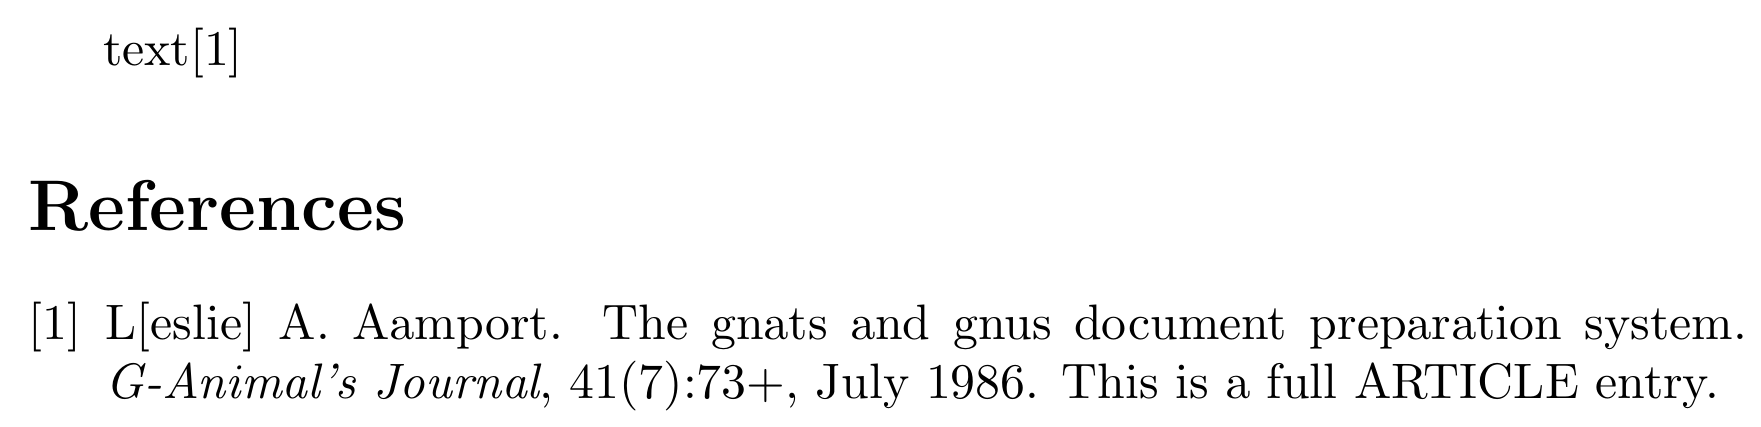
\includegraphics[width=\textwidth]{bib-ref.png}
  \end{center}
\end{onlyenv}
\end{frame}

\subsubsection{更强大的工具: \texttt{latexmk}}

\begin{frame}[fragile]
  \frametitle{使用命令行编译 \LaTeX 文件}
  \framesubtitle{更强大的工具: \texttt{latexmk}}

\begin{latexcode}
% main.tex
\documentclass{ctexart}
\usepackage[style=gb7714-2015]{biblatex}
\addbibresource{xampl.bib}
\begin{document}
\tableofcontents
\section{测试节}\label{sec:one}
  我们现在是第 \ref{sec:one} 节,
  我们有一个引用 \cite{article-full}
  \printbibliography
\end{document}
\end{latexcode}

\begin{cmdcode}
latexmk -xelatex main.tex
\end{cmdcode}


\end{frame}

\subsubsection{更多}

\begin{frame}{使用命令行编译 \LaTeX 文件}
  \framesubtitle{更多的内容}
  latexmk 命令文件
  \begin{itemize}
    \item \cmd{latexmk -c}, \cmd{latexmk -C};
    \item \texttt{latexmkrc} 文件.
  \end{itemize}
  
  更多内容可以参见
  \begin{itemize}
    \item \texttt{\textbf{texdoc} latexmk}
    \item \cmd{pdflatex --help}
    \item \href{https://syvshc.github.io/2022-03-06-latex-terminal-compiling/}{在终端中编译 \LaTeX}
  \end{itemize}
\end{frame}

\section{使用 \tlmgr 进行包管理}

\begin{frame}[fragile]{\tlmgr 命令介绍}
\begin{itemize}
  \item \tlmgr 是 \texlive 用来管理\emph{软件包}的工具;
  \item \emph{软件包}指的不只是可以通过 \lcmd{\usepackage} 调用的宏包, 而是所有 \texlive 包含的, 可以使用 \tlmgr 管理的内容, 比如平常所说的宏包, 如 \lstinline{amsmath.sty}, 一些说明文档, 如 \lstinline{lshort-zh-cn}, 一些可执行文件, 如 \lstinline{xetex.exe} 等等.
  \item \tlmgr 是 \textbf{T}eX\textbf{L}ive \textbf{M}ana\textbf{g}e\textbf{r} 的缩写;
  \item 命令行中运行 \cmd{tlmgr version} 就可以看到当前的\emph{修订版号}(revision), 通常输出如下
  \begin{outputcode}
  tlmgr revision 63033 (2022-04-15 07:19:42 +0200)
  tlmgr using installation: C:/texlive/2022
  TeX Live (https://tug.org/texlive) version 2022
  \end{outputcode}
\end{itemize}
\end{frame}


\begin{frame}[fragile]{\tlmgr 的基本语法}
\begin{cmdcode}
tlmgr -global-options action -action-specific-options operand
\end{cmdcode}
\begin{enumerate}
  \item \cmd{-} 与 \cmd{--} 相同;
  \item 顺序不重要;
  \item \cmd{-dry-run}.
\end{enumerate}
\end{frame}


\begin{frame}[fragile]{查看宏包文件信息 --- 操作: \frameaction{info}}

\begin{cmdcode}
tlmgr info -list pkg1 pkg2
\end{cmdcode}
\begin{outputcode}
# 省略 tlmgr info tabularray 的内容 #
Included files, by type:
run files:
texmf-dist/tex/latex/tabularray/tabularray-2021.sty
texmf-dist/tex/latex/tabularray/tabularray.sty
doc files:
texmf-dist/doc/latex/tabularray/README.txt details="Readme"
texmf-dist/doc/latex/tabularray/tabularray.pdf details="Package documentation"
texmf-dist/doc/latex/tabularray/tabularray.tex  
\end{outputcode}
\end{frame}


\begin{frame}[fragile]{查看宏包说明信息 --- 操作: \frameaction{info}}
\begin{cmdcode}
tlmgr info pkg1 pkg2
\end{cmdcode}
\begin{outputcode}
package:     ctex
category:    Package
shortdesc:   LaTeX classes and packages for Chinese typesetting
longdesc:    ctex is a collection of macro packages and document classes for LaTeX Chinese typesetting.
installed:   Yes
revision:    61285
sizes:       src: 481k, doc: 1137k, run: 1753k
relocatable: No
cat-version: 2.5.8
cat-license: lppl1.3c
cat-topics:  chinese book-pub class
cat-contact-bugs: https://github.com/CTeX-org/ctex-kit/issues
cat-contact-support: https://github.com/CTeX-org/ctex-kit/issues
cat-contact-repository: https://github.com/CTeX-org/ctex-kit
cat-contact-home: http://www.ctex.org/HomePage
collection:  collection-langchinese
\end{outputcode}
\end{frame}

\begin{frame}[fragile]{修改宏包更新源 --- 操作: \frameaction{option}}

\begin{cmdcode}
tlmgr option repository mirror
\end{cmdcode}

值得一提: \cmd{repository} = \cmd{repo}
\end{frame}

\begin{frame}[fragile]{更新软件包 --- 操作: \frameaction{update}}
\framesubtitle{查看哪些软件包可以更新}

\begin{cmdcode}
tlmgr update -list
\end{cmdcode}
\begin{outputcode}
tlmgr.pl: package repository https://mirrors.tuna.tsinghua.edu.cn/CTAN/systems/texlive/tlnet (not verified: gpg unavailable)
tlmgr.pl: would save backups to C:/texlive/2022/tlpkg/backups
tlmgr.pl: skipping forcibly removed package: collection-texworks
update:   adjmulticol   [316k]: local:  62935, source:  63073
update:   hitex         [2565k]: local:  62529, source:  63073
update:   texlive-fr    [1394k]: local:  62853, source:  63071
update:   texlive-msg-translations [144k]: local:  63010, source:  63072
update:   texlive-scripts.win32 [36k]: local:  62199, source:  63068
update:   texlive-scripts [504k]: local:  63049, source:  63068
update:   utfsym         [4766k]: local:  56729, source:  63076
update:   xduts          [871k]: local:  63013, source:  63075
update:   zwpagelayout   [641k]: local:  53965, source:  63074  
\end{outputcode}
\end{frame}

\begin{frame}[fragile]{更新软件包 --- 操作: \frameaction{update}}
\framesubtitle{更新全部软件包}

\begin{cmdcode}
tlmgr update -self -all
\end{cmdcode}
\begin{outputcode}
tlmgr.pl: package repository https://mirrors.tuna.tsinghua.edu.cn/CTAN/systems/texlive/tlnet (not verified: gpg unavailable)
tlmgr.pl: saving backups to C:/texlive/2022/tlpkg/backups
tlmgr.pl: no self-updates for tlmgr available
[ 1/16, ??:??/??:??] update: babel-french [567k] (59997 -> 63088) ... done
[ 2/16, 00:02/01:48] update: l3backend [894k] (63025 -> 63089) ... done
...
[16/16, 01:23/01:23] update: collection-luatex [1k] (62829 -> 63081) ... done
running mktexlsr ...
done running mktexlsr.
running mtxrun --generate ...
done running mtxrun --generate.
running updmap-sys ...
...
tlmgr.pl: package log updated: C:/texlive/2022/texmf-var/web2c/tlmgr.log
tlmgr.pl: command log updated: C:/texlive/2022/texmf-var/web2c/tlmgr-commands.log
\end{outputcode}
\end{frame}

\begin{frame}[fragile]{更新软件包 --- 操作: \frameaction{update}}
\framesubtitle{其他的功能}
\begin{enumerate}
\item 更新软件包 \pkg{pkg1}, \pkg{pkg2}:
\begin{cmdcode}
tlmgr update pkg1 pkg2
\end{cmdcode}
\item 如果更新全部宏包时不想更新 \pkg{pkg1}, \pkg{pkg2}:
\begin{cmdcode}
tlmgr update -self -all -exclude pkg1 -exclude pkg2
\end{cmdcode}
\item 如果更新过程被中断
\begin{cmdcode}
tlmgr update -self -all -reinstall-forcibly-removed
\end{cmdcode}
\end{enumerate}
\end{frame}


\subsection{回滚软件包的版本}

\begin{frame}[fragile]
  \frametitle{回滚软件包的版本 --- 操作: \frameaction{restore}}
  
  \framesubtitle<1>{查看某个软件包的备份} 
  % \begin{onlyenv}<1>
\begin{cmdcode}
tlmgr restore pkg
\end{cmdcode}
\begin{outputcode}
tlmgr restore functional
Available backups for functional: 62926 (2022-04-17 11:15)
\end{outputcode}
  % \end{onlyenv}
  \framesubtitle<2>{将某个软件包回滚为备份}

\begin{uncoverenv}<2>
\begin{cmdcode}
tlmgr restore pkg revision
\end{cmdcode}
\begin{outputcode}
tlmgr restore functional 62926
Do you really want to restore functional to revision 62926 (y/N): y
Restoring functional, 62926 from C:/texlive/2022/tlpkg/backups/functional.r62926.tar.xz
running mktexlsr ...
done running mktexlsr.
running mtxrun --generate ...
done running mtxrun --generate.
tlmgr.pl: package log updated: C:/texlive/2022/texmf-var/web2c/tlmgr.log
tlmgr.pl: command log updated: C:/texlive/2022/texmf-var/web2c/tlmgr-commands.log
\end{outputcode}
\end{uncoverenv}
\end{frame}

\subsection{更多内容}

\begin{frame}
  \frametitle{更多内容}
  如果想了解更多关于 tlmgr 的信息, 欢迎阅读我翻译的 \href{http://mirrors.ctan.org/info/tlmgr-intro-zh-cn/tlmgr-intro-zh-cn.pdf}{tlmgr-intro-zh-cn} 以及 \href{https://www.tug.org/texlive/doc/tlmgr.html}{tlmgr 的官方文档}
\end{frame}




\subsection{检查宏包是否安装}

\begin{frame}[fragile]
  \frametitle{安装外部宏包}
  \framesubtitle{检查一个宏包是否被安装了}
\begin{cmdcode}
tlmgr info pkg
# or 
kpsewhich pkg.sty
\end{cmdcode}
\end{frame}

\begin{frame}[fragile]{安装外部宏包}
\framesubtitle{手动安装宏包}

\begin{enumerate}
  \item 下载或者编写一个宏包文件(cls) 
    \begin{latexcode}
    % mypackage.sty
    \NeedsTeXFormat{LaTeX2e}[2017/04/15]
    \ProvidesPackage{mypackage}[2022/4/20 v1.0 test]
    \newcommand{\mycmd}{Hello \LaTeX}  
    \end{latexcode}
  \item 在 \directory{C:/texlive/texmf-local/tex/latex} 文件夹下新建文件夹 \directory{mypackage};
  \item 将 \texttt{mypackage.sty} 放进去;
  \item 命令行运行 \cmd{texhash}.
  \item 调用该宏包:
  \begin{latexcode}
    % main.tex
    \documentclass{article}
    \usepackage{mypackage}
    \begin{document}
      \mycmd
    \end{document}
    \end{latexcode}
\end{enumerate}
\end{frame}


\section{VS Code 的安装与配置}
\subsection{下载并安装 VSCode}
\begin{frame}[fragile]{VS Code 安装 --- Windows 用户}
  \begin{itemize}
    \item 在 VSCode 的官网 \href{https://code.visualstudio.com/}{https://code.visualstudio.com/} 选择 stable 版本进行下载
    \item 安装的时候注意将 ``通过 Code 打开'' 添加到上下文菜单:
  \end{itemize}

  \begin{center}
    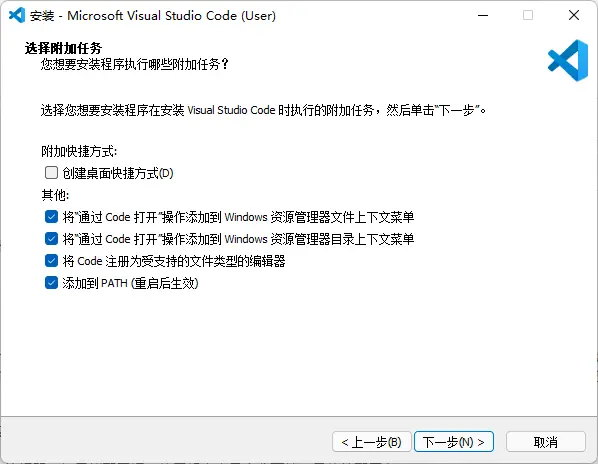
\includegraphics[width=8cm]{install-vs.png}
  \end{center}

\end{frame}

\begin{frame}{基础设置与 LaTeX Workshop 安装}
  \begin{enumerate}
    \item 更改语言为中文
    \item 安装 LaTeX Workshop
    \item 配置 LaTeX Workshop 编译链
    \item 更多内容:参见 \href{https://gitee.com/xkwxdyy/CCNUthesis/wikis/\%E5\%B8\%B8\%E8\%A7\%81\%E9\%97\%AE\%E9\%A2\%98FAQ/\%E5\%A6\%82\%E4\%BD\%95\%E5\%AE\%89\%E8\%A3\%85\%E3\%80\%81\%E9\%85\%8D\%E7\%BD\%AE\%E5\%92\%8C\%E4\%BD\%BF\%E7\%94\%A8VScode\#config-LW}{Wiki}. 
  \end{enumerate}
\end{frame}